\chapter{Hull-White Single-Factor Model}
\label{chapter:hullwhitemodel}
The following chapter will study the Hull-White Single-Factor Model to understand the algorithm behind it and prepare a strategy for a parallel implementation. It will first introduce a general overview of how a trinomial tree is being constructed, and later show how prices are being discounted from it. 

\section{Hull-White Trinomial Tree}
In this project, we implement the trinomial tree numerical method to discretize the Hull-White model.  In contrast to the standard trinomial tree, the tree used in the Hull-White model incorporates the mean-reversion of the interest rate, by using a width limit and modified branching methods for the tree. Standard branching (see fig.~\ref{fig:background:standardbranching}) remains the same throughout the tree. At the bottom of the tree, where interest rates are very low, the \enquote{up one/straight along/down one} (see fig.~\ref{fig:background:altbranchingbottom}) branching is used. At the top of the tree, where interest rates are very high, the \enquote{straight along/down one/down two} branching is used (see fig.~\ref{fig:background:altbranchingtop}). 

\begin{figure}
\centering
\begin{subfigure}{.3\textwidth}
  \centering
  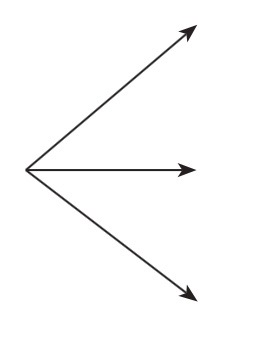
\includegraphics[width=.7\linewidth]{img/standardbranch.jpg}
  \caption{Standard branching}
  \label{fig:background:standardbranching}
\end{subfigure}
\begin{subfigure}{.3\textwidth}
  \centering
  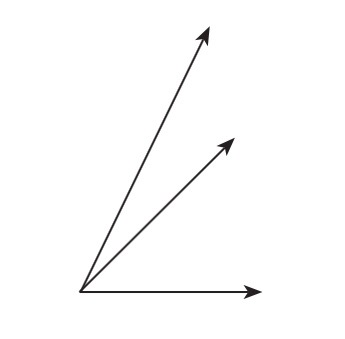
\includegraphics[width=.93\linewidth]{img/bottombranch.jpg}
  \caption{Bottom branching}
  \label{fig:background:altbranchingbottom}
\end{subfigure}
\begin{subfigure}{.3\textwidth}
  \centering
  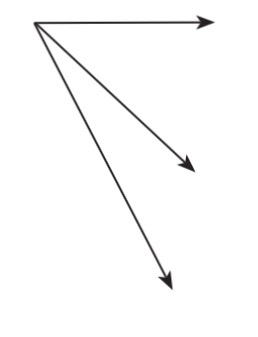
\includegraphics[width=.7\linewidth]{img/topbranch.jpg}
  \caption{Top branching}
  \label{fig:background:altbranchingtop}
\end{subfigure}
\caption{Alternative branching methods for a trinomial tree.}
\label{fig:background:allbranchings}
\source{Based on Options, Futures and Other Derivatives\cite[pg. 698]{ofod}.}
\end{figure}

We observe that this pruning characteristic allows us to asses the size of the tree upfront and use this knowledge to enable more specific implementation optimizations, in particular how to map the tree to the parallel device thread and memory architecture. Otherwise, the tree could grow infinitely in its width, making it impossible to map to limited parallel architecture memory resources and invalidating certain parallel implementations.

\section{Overview}
Pricing a single option using Hull-White short-rate\footnote{The short rate, \textit{r}, at time \textit{t} is the rate that applies to an infinitesimally short period of time at time \textit{t}\cite[pg. 682]{ofod}} single-factor trinomial tree model enables the term structure of interest rates at any given time to be obtained from the value of the short rate \textit{r} at that time and the risk-neutral process for \textit{r}. This shows that, once the process for \textit{r} has been defined, everything about the initial zero curve and its evolution through time can be determined\cite[pg. 683]{ofod}. 
\\\\
The model consists of two steps. The first (forward propagation along the tree) is the construction of the trinomial tree in order to obtain a list of alpha values for each time step. These alphas are later used in the second step (backward propagation along the tree) to fit the option/bond prices and obtain the option value back at the root node of the tree. The input fed to the algorithm consists of an option, which includes its strike price, maturity, time step length, mean-reversion rate\footnote{denoted as $a$ - determines the relative volatilities of long and short rates\cite[pg.9]{npfits}} and volatility\footnote{denoted as $\sigma$ - determines the overall level of volatility \cite[pg. 9]{npfits}}. The output is the estimated price of the option/bond. The two steps can be generalized as follows: 

\begin{enumerate}
    \item \textbf{Forward propagation step:} Construct a term structure for the underlying asset by progressing one time step at a time. Determine neutral risk rate for a new time step using estimated yield curve data and estimated current asset values.
    \item \textbf{Backward propagation step:} Discount the asset prices to estimate option payoff at maturity going from the leaves of the tree to its root. 
\end{enumerate}

Algorithm~\ref{alg:loops} shows a high-level overview of a function implementing this procedure for pricing one option. The input of the algorithm is an option and a yield curve (used for the computation of alphas) and the output is the estimated price of the option. The function consists primarily of two sequential (convergence) loops of count tree height, which contain inner parallel operators of count tree width, where tree height and width are specific to each option (and thus vary across options). The tree height is dependent on the number of time steps, i.e., maturity of the underlying bond and precision. The tree width is dependent on the number of terms and input parameters.

Different option/bond maturities (leading to different tree heights) and different level of pricing accuracy (number of simulated time steps leading to different tree dimensions) make the choice of an effective parallelization strategy difficult. It is necessary to have a deep understanding of the algorithm itself to achieve maximum parallelization efficiency. The book by John Hull\cite{ofod} provides a solid background on the topic, describing the mechanics of interest rates, markets, as well as application of binomial trees and eventually trinomial trees to option pricing. Chapter 30 further narrows the topic of using trinomial trees as a numerical method and introduces a step by step walk-through of applying the algorithm on a basic example. While some of the calculation details are omitted in the book, the authors provide references to previous articles\cite{npfits}\cite{uhwirt}, where they provide a thorough explanation backed with more detailed examples. 

\newpage
It is important to mention that the construction of a trinomial tree is a discrete-time, lattice-based\footnote{A model that takes into account expected changes in various parameters e.g. interest rate over the duration of the option} numerical method, but the example in the book is simplified by cutting the tree at a certain height and using analytic formulas to produce a concrete result for a specific financial instrument - a zero-coupon bond maturing at time $(m + 1) * \triangle t$ \cite[pg. 704]{ofod}. These formulas have been found and proven to be effective by the authors of the book and the articles. While this simplification gives more precise results in the above mentioned specific case, constructing the entire tree and using all of the time steps provides a foundation for pricing other options with more sophisticated cashflows. All the implementations of this thesis will be focused on the described numerical approach.

The following sub-chapters are focused primarily on the intuition behind the algorithm, with the sole purpose to provide the reader with a general overview for it. For this reason, many of the details and formulas of calculating specific values are omitted, however they are thoroughly described in the book and the articles by Hull and White. As the model is best understood visually, we have included some of the supplementary images from the Hull and White book in order to support our algorithm explanation.

\newpage
\begin{algorithm}[H]
\DontPrintSemicolon
\caption{High-level overview of pricing a single option using Hull-White Single-Factor Model\label{alg:loops}}
\SetKwInOut{Input}{Input}
\SetKwInOut{Output}{Output}

\Input{Option, YieldCurve}
\Output{Price approximation}
\;
alphas[0] = Compute yield at initial interest rate\;
Qs[0][$\text{width}/2$] = 1\tcc*{Initialize the root node to 1\textdollar}
\;
\tcc{Forward propagation (convergence) loop}
\For{$i = 0$ \KwTo height} {
    \tcc{Compute Qs at the next time step}
    \For{$j = 0$ \KwTo width} {
        Qs[$\text{i} + 1$][j] = Compute Q from Qs[i] and alphas[i]\;
    }
    Compute alphas[$\text{i} + 1$] from Qs[i]\;
}
\;
\tcc{Initialize prices at the last time step to 100\textdollar}
Prices[$\text{height} - 1$] = 100\;
\;
\tcc{Backward propagation (convergence) loop}
\For{$i = \mathit{height} - 1$ \KwTo 0} {
    \tcc{Compute prices at the previous time step}
    \For{$j = 0$ \KwTo width} {
        Prices[i][j] = Compute price from Prices[$\text{i}+1$] using alphas[i]\;
    }
}
\;
\tcc{Return price at the root node}
\Return Prices[0][$\text{width}/2$]\;
\end{algorithm}

\section{Forward Propagation}
\label{section:hullwhite:forwardpropagation}
The forward propagation by itself consists of two stages. Each of them computes different values on the same tree. While the tree height can grow indefinitely, depending on the number of time steps, the width of the tree is limited by mean-reversion (as reasoned for in chapter \ref{chapter:background}), by determining its max. width (or as we refer to it for simplicity - width). 

\paragraph{Indexing} Since the tree is 2-dimensional, locating and computing values on individual nodes boils down to locating them by index first. Hence, we introduce the two indexes - \textit{i} and \textit{j}, used to indicate the tree height and its width respectively. To describe the meaning of \textit{i} and \textit{j} visually, we can use fig. \ref{fig:treeconststage1}, where nodes along the height - A, C, G - can be indexed as i = 0, 1, 2. Indexing across the width is different, as we intuitively denote the core of the tree - nodes A, C, G - with $j=0$. Going down along the three decreases the value of $j$, while going up increases it. This means that nodes D,H are located on $j=-1$, nodes B,F are located on $j=1$ and so on. We denote the highest node across the width as $j_{max}$ and $j_{min}$ as the lowest. Note that $j_{min}=-j_{max}$ due to the symmetry of the tree, making it possible to omit $j_{min}$ occurrences in our implementations by replacing them with $-j_{max}$. On fig. \ref{fig:treeconststage1} nodes E and I are at the top and at the bottom of the tree width, hence their $j$ indexes are equal to $j_{max}$ and $j_{min}$ respectively. The index values in this example are $j_{max}=2$ and $j_{min}=-2$. Note that our code cannot always be aligned with our intuition and indexes cannot be negative in our programs. Hence we can shift the indexing between $j_{min}$ and $j_{max}$ and count from $0$ to $2*j_{max}+1$ instead, making the root node to be located at index $j_{max}$. Despite that, we have used $j_{min}$ and $j_{max}$ as width boundaries throughout this report, as they are easier to comprehend.

\paragraph{Stage 1}
aims to construct a tree for a variable $R^*$ that is initially 0 and follows the Ornstein–Uhlenbeck stochastic\footnote{With a random probability distribution or pattern that may be analyzed statistically but may not be predicted precisely.} process\footnote{Tends to drift towards its long-term mean (also called mean-reverting).} $dR^*=-aR^*dt + \sigma dz$ which is symmetrical about $R^*=0$\cite[pg.698-699]{ofod}. Together with $R^*$, $p_u$, $p_m$ and $p_d$ are calculated to match the respective up, mid and down probabilities that match the expected change and variance of the change in R over the next interval $\triangle t$. Since the width of the tree is limited between $j_{min}$ and $j_{max}$, some of the branching is calculated differently, thus $p_u$, $p_m$ and $p_d$ depend on the node position. Naturally the tree construction happens iteratively, node by node, starting from the root. In the end of the stage, this first tree will always have a symmetrical shape\footnote{Trinomial trees are recombining, meaning that at any time, an up move followed by a down move has exactly the same effect on the price as a down move followed by an up move.} similar\footnote{Note that the width and height of the tree may differ based on the number of time steps and the maturity of the financial instrument} to fig.\ref{fig:treeconststage1}. 
\begin{figure}[H]
	\centering
	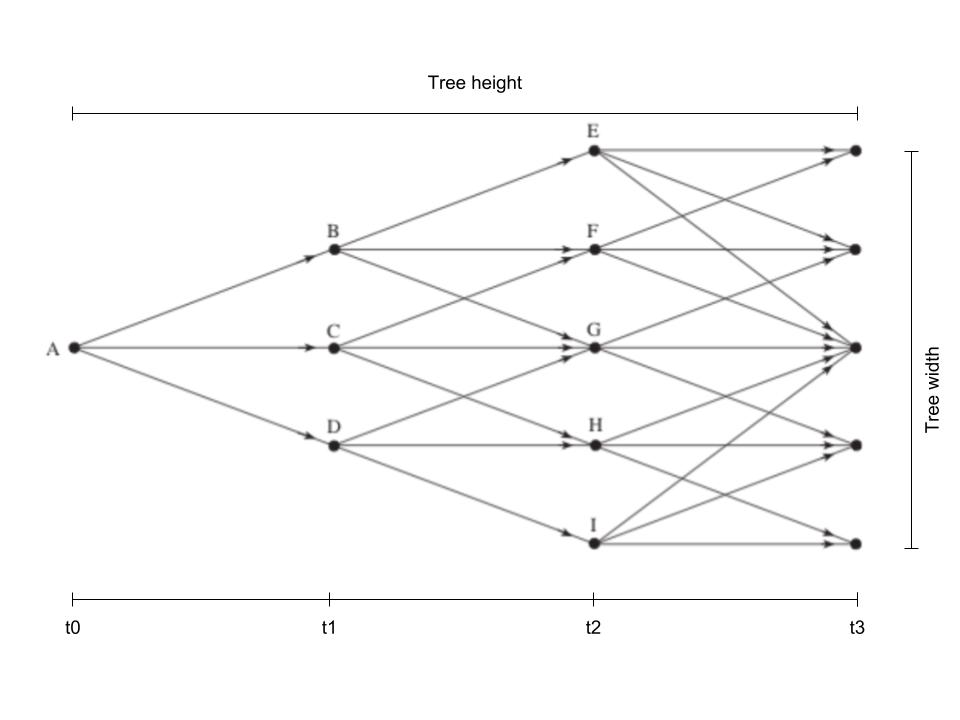
\includegraphics[width=0.8\textwidth]{img/treeconststage1wh.jpg}
	\caption{Example of the trinomial tree for $R^*$.}
	\source{Modified by the authors, based on Options, Futures and Other Derivatives\cite[pg. 699]{ofod}.}
	\label{fig:treeconststage1}
\end{figure}

An important property of this tree include first of all that it is self-recombining, causing it to be symmetric. The probabilities on the lower part of the tree will be the negative of the probabilities on the upper part of the tree, e.g. probability that node A reaches node D is minus the probability of node A reaching node B. Furthermore, also due to symmetry, all unique probabilities can be stored in an array of size the width of the tree, because e.g. the probability of node A reaching node B is the same as the probability of node C reaching node F and so on. Probabilities are used both in stage 2 of the forward propagation, but also in the backward propagation, thus it is necessary to contain them to the end, if they are to be stored. Last but not least, the way probabilities are calculated is different on $j_{min}$ or $j_{max}$, because of the difference in branching. This can be seen on fig. \ref{fig:treeconststage1} where nodes E and I branch out differently in comparison to all other nodes. 

\paragraph{Stage 2}
In this stage, the rates at each node in the tree at each time step are shifted up by an amount - $\alpha$, chosen so that the revised tree correctly prices discount bonds \cite[pg. 6]{uhwirt}. This is done by defining $Q_{i,j}$ as the present value of a security that pays off \$1 if node (i, j) is reached and 0 otherwise. The starting point is to set $Q_{0,0}=0$ and $\alpha_0$ to the interest rate at time $\triangle t$. $Q$s at the next time step are then calculated by using the generalized formula \cite[pg.705]{ofod}:  
\begin{equation}
\begin{gathered}
\begin{aligned}
Q_{m+1, j} = \sum_k Q_{m,k}q(k,j)exp[-(\alpha_m+k\triangle r)\triangle t]
\nonumber
\end{aligned}
\end{gathered}
\end{equation}
Assuming that we start at step $m$, to calculate the $Q$s on step $m+1$, we need to have the $\alpha$ on step $m$. Furthermore, once the $Q$s on step $m+1$ have been calculated, they are used to also find the $\alpha$ on $m+1$ later. This leads to conclude that $\alpha$s and $Q$s are interrelated on each time step. $\alpha$s are calculated using the generalized formula \cite[pg.703]{ofod}:
\begin{equation}
\begin{gathered}
\begin{aligned}
\alpha_{m} = \dfrac{\sum_{j=-n_m}^{n_m} Q_{m,j}e^{-j\triangle r\triangle t} - \ln{P_{m + 1}}}{\triangle t}
\nonumber
\end{aligned}
\end{gathered}
\end{equation}
At the end of this stage, the new tree will have changed visually. For example, the tree from fig. \ref{fig:treeconststage1} can be re-shaped as shown on fig. \ref{fig:treeconststage2}. 
\begin{figure}[H]
	\centering
	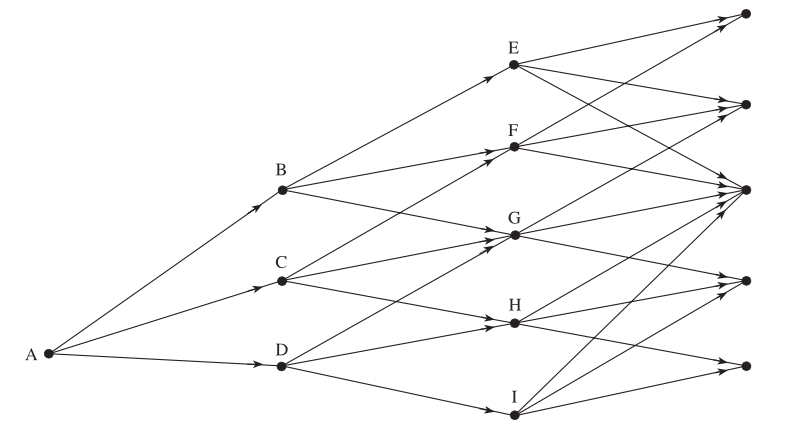
\includegraphics[width=0.8\textwidth]{img/treeconststage2.png}
	\caption{Example of the trinomial tree for $R$.}
	\source{Options, futures and other derivatives fig. 30.9 \cite[pg. 702]{ofod}}
	\label{fig:treeconststage2}
\end{figure}
An important observation here is that the only outcome of this tree that is used in the backward propagation is the array of $\alpha$s. $Q$s are in this case intermediary values, used to compute the $\alpha$ on each step and for this reason, the $Q$ values do not need to be stored any longer once all $\alpha$s have been computed. 

\section{Backward Propagation}
The backward propagation starts with the previously constructed tree during the forward propagation step, in particular with array of $\alpha$s. At each time-step the option payoff is computed as the discounted value of the expected value at the next step \cite[pg. 6]{uhwirt}. From this it follows that the nodes at time step $i$ (e.g. the nodes without assigned letters in figures \ref{fig:treeconststage1} and \ref{fig:treeconststage2} above) are the starting point of the backward propagation. Their values are set to 100\$ and are used to compute the previous set of nodes (at time step $i-1$). That is done by discounting bond price values up until the exercise of the option. At the option expiration time step, we decide if we exercise the option or let it expire worthless. To achieve that, we calculate the difference between bond price and the strike price. The positive values mean exercise, while non-positive mean expiry worthless and are set to $0$. We discount the option prices further down to the root of the tree to get the approximation of the option price on the valuation day. This is the output of the algorithm. We use the array of $\alpha$s computed during the forward propagation through this procedure. It is important to note that determining the option price depends on the type of option (whether it is a put or a call option).

\section*{Summary}
This chapter has provided a detailed overview of the Hull-White Single-Factor Model, in particular its two-stage procedure fo propagating along a trinomial tree. It will be used in the following chapter, which will introduce the challenges of implementing a sequential version of the algorithm in C++.
